\documentclass{beamer}

\usepackage{graphicx,url}
\usepackage[brazil]{babel}
\usepackage[utf8]{inputenc}
\usepackage{mathtools}
\usepackage{fix-cm}
\usepackage{eucal}
\usepackage{amscd}
\usepackage{amsmath}
\usepackage{amssymb}
\usepackage{listings}
\usepackage{colortbl}
\usepackage{latexsym}
\usepackage{verbatim}
\usepackage{hyperref}
\usepackage{booktabs}
\usepackage{subfig}

\mode<presentation> {
  \usetheme{Madrid}

  \usecolortheme{orchid}

  \setbeamertemplate{navigation symbols}{}
}

\title[Decidibilidade e Redução de Problemas]{Decidibilidade e Redução de Problemas}

\author{Ramon Santos Nascimento}

\institute[UFRPE]{
  \centering 
\includegraphics[width=1.6cm]{img/logo.png}\\

  \medskip
  Universidade Federal Rural de Pernambuco \\
  \medskip

  \textit{ramonsantos.pe@gmail.com}
}

\date{27 de Janeiro de 2014}

\newcommand{\ok}{$\surd$}

\begin{document}
  \begin{frame}
    \titlepage
  \end{frame}

  \begin{frame}{Decidibilidade}
    \begin{block}{Definição}
      \begin{itemize}
        \item Um problema é decidível se sua solução é encontrada por uma \textbf{Máquina de Turing} que retorna uma resposta;

        \item Caso contrário, o problema é indecidível.
      \end{itemize}
    \end{block}
  \end{frame}

  \begin{frame}{Problema de aceitação - Linguagens recursivas}
    Seja $U$ uma $M.T.U.$ com entrada $<M, \omega>$:\newline

    \begin{itemize}
      \item \textbf{ACEITA}: Se $M$ em algum momento entra no seu estado de aceitação;

      \item \textbf{REJEITA}: Se $M$ em algum momento entra em estado de rejeição.\newline
    \end{itemize}

    É decidível.
  \end{frame}

  \begin{frame}{Problema de aceitação - Linguagens recursivamente enumeráveis}
    Seja $U$ uma $M.T.U.$ com entrada $<M, \omega>$:\newline

    \begin{itemize}
      \item \textbf{ACEITA}: Se $M$ em algum momento entra no seu estado de aceitação;

      \item \textbf{REJEITA}: Se $M$ em algum momento entra em estado de rejeição ou se $M$ entra em loop.\newline
    \end{itemize}

    É indecidível.
  \end{frame}

  \begin{frame}{Hierarquia de Chomsky}
    \begin{figure}[ht]
      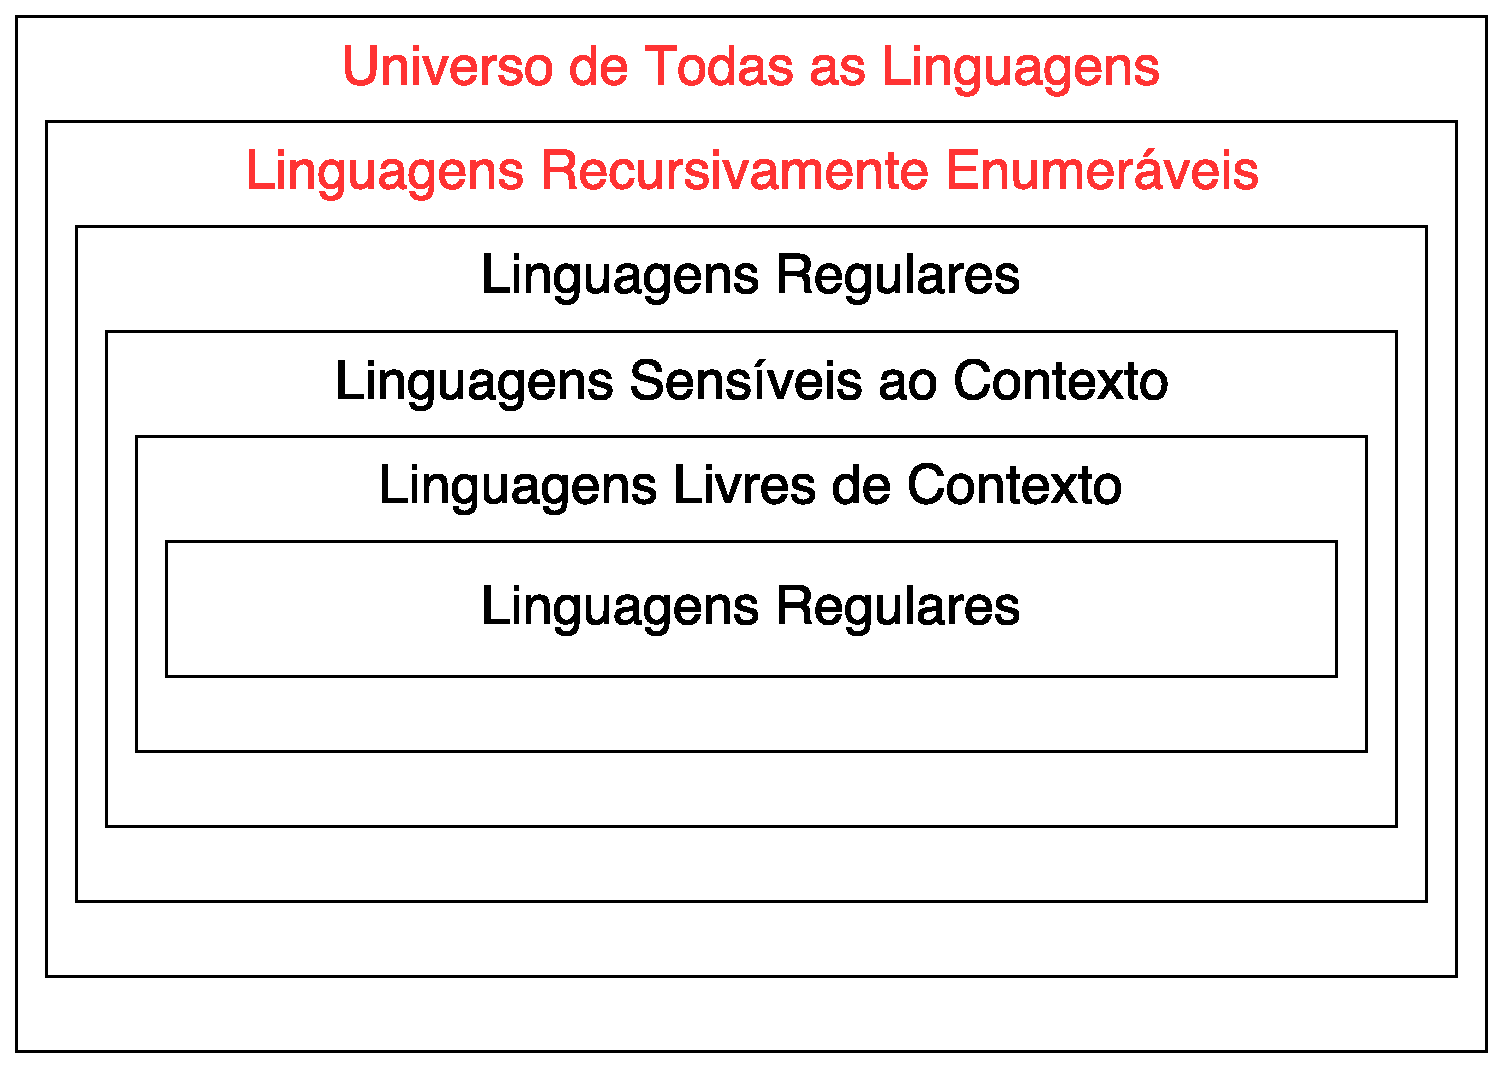
\includegraphics[width=0.80\textwidth]{img/hierarquia-Chomsky.pdf}
    \end{figure}
  \end{frame}

  \begin{frame}{Redutibilidade}
    \begin{block}{Definição}
      É uma maneira de converter um problema em outro de forma que uma solução para o segundo problema possa ser usada para resolver o primeiro.
    \end{block}
  \end{frame}

  \begin{frame}{Redutibilidade}
    Sejam os problemas $A$ e $B$.\newline

    Se $A$ se reduz a $B$, podemos usar uma solução de $B$ para resolver $A$.\newline

    \begin{block}{Teorema 1}
      Se $A$ é redutível a $B$ ($A \le B$) e $B$ é decidível então $A$ é decidível.
    \end{block}

    \begin{block}{Teorema 2}
      Se $A$ é redutível a $B$ ($A \le B$) e $A$ é indecidível então $B$ é indecidível.
    \end{block}
  \end{frame}

  \begin{frame}{Redutibilidade por mapeamento}
    Significa que existe uma função computável que converte instâncias do problema $A$ para instâncias do problema $B$.\newline

    Sejam as Linguagens $A$ e $B$, $A$ é redutível por mapeamento à $B$ ($A \le_{m} B$), se existe uma função computável $f : \sum^{*} -> \sum^{*}$, onde para toda $\omega$,\newline

    \begin{align*}
      \omega \in A \leftrightarrow f(\omega) \in B
    \end{align*}
  \end{frame}

  \begin{frame}{A importância dos assuntos}
    \begin{itemize}
      \item Saber se um problema é decidível.
        \begin{itemize}
          \item E se não for, o que fazer?\newline
        \end{itemize}

      \item Usar Redutibilidade para provar que um problema é indecidível.
        \begin{itemize}
          \item Como?\newline
        \end{itemize}

      \item Usar Redutibilidade para resolver problemas.
        \begin{itemize}
          \item Como?\newline
        \end{itemize}
    \end{itemize}
  \end{frame}

  \begin{frame}{Dúvidas}
    \Huge{\centerline{Dúvidas?}}
  \end{frame}

  \begin{frame}{Obrigado}
    \Huge{\centerline{Obrigado!}}
  \end{frame}
\end{document}
